\documentclass[aspectratio=169]{beamer}

%includeonlyframes{current}

\usepackage[T1]{fontenc}
\usepackage[utf8]{inputenc}
\usepackage[american]{babel}
\usepackage{amsmath,amsthm}
\usepackage{multirow}
\usepackage{tikz}
\usetikzlibrary{matrix,decorations,decorations.text,calc,arrows,snakes,shapes,positioning}
\usepackage{multimedia}

\usepackage[nosfdefault]{comicneue}
\usepackage{sourcesanspro}
\usepackage[amssymb,amsfonts]{concmath}
\usefonttheme[onlymath]{serif}
\usepackage{ulem}

\mode<presentation>{%
  \usetheme{ibm}
}

\newcommand{\F}{\mathbb{F}}
\newcommand{\Z}{\mathbb{Z}}
\newcommand{\Q}{\mathbb{Q}}
\DeclareMathOperator{\End}{End}
\DeclareMathOperator{\Cl}{Cl}
\DeclareMathOperator{\poly}{poly}
\DeclareMathOperator{\polylog}{polylog}


\title{Delay Assumptions in Cryptography}
\author[Luca De Feo]{
  Luca De Feo\\[1em]
  based on joint work with J.~Burdges, S.~Masson, C.~Petit, A.~Sanso}
\date{April 16, 2020, ZRL Security Seminar}
\institute{IBM Research Zürich}

\begin{document}

\frame[plain]{\titlepage}

%% 

\begin{frame}{Computational hardness in cryptography}
  \begin{center}
    \framebox{\textcolor{gray}{boring picture of Alice, Bob and Eve goes here}}
  \end{center}

  \medskip
  
  \textbf{\emph{How long} will it take Eve to decrypt the message?}
  \smallskip
  \begin{description}
  \item[Complexity theory:] (sub)exponentially more than Bob.
    \begin{itemize}
    \item Asymptotics don't say anything on constants.
    \item Based on a \emph{best-case} analysis, ignores \emph{average}
      and \emph{worst case}.
    \item Typically based on a Turing-machine-like model, doesn't
      necessarily fit reality.
    \end{itemize}
  \item[Real world crypto:] at least $2^{128}$ ``operations''.
    \begin{itemize}
    \item But what's an ``operation''?
    \item Often based on extrapolations (see, in particular, factoring).
    \item Doesn't account for parallelism.
    \item More a measure of \emph{cost} than a measure of \emph{time}.
    \end{itemize}
  \end{description}
\end{frame}

%%

\begin{frame}{Time-lock Puzzles}
  \begin{center}
    \begin{tikzpicture}
      \node (fred) at (0,0) {\includegraphics[height=6em]{fred.png}};
      \node (jets) at (9.2,0) {\includegraphics[height=7em]{jetsons.png}};
      
      \foreach \i in {2,...,6} {
        \pgfmathparse{int(14-2*\i)}
        \let\time\pgfmathresult
        \uncover<\i>{
          \draw (\i,0.5) node {\includegraphics[width=2em]{chest-closed.png}};
          \draw (4.6,-0.5) node {\comicneue\bfseries\footnotesize OPEN IN \time 00000 YEARS};
          \draw[thick,->] (fred) edge (\i+1,0);
        }
      }
      \uncover<7>{
        \draw (7,0.5) node {\includegraphics[width=2em]{chest-open.png}};
        \draw (4.6,-0.5) node {\comicneue\bfseries\footnotesize YABBA DABBA DOO!};
        \draw[thick,->] (fred) edge (8,0);
      }
    \end{tikzpicture}
  \end{center}

  Basically a \emph{Key Derivation Function} (family) with two
  algorithms: \medskip
  \begin{description}
  \item[KDF$(T, \Delta)$:] which computes a \emph{key} $k$
    given a \emph{trapdoor} $T$ and a \emph{delay} $\Delta$.
  \item[SlowKDF$(\Delta)$:] which computes the same key $k$
    without knowledge of the trapdoor,\\
    \emph{in time approximately $\Delta\cdot\mathrm{constant}$}.
  \end{description}
  \smallskip \dots under the conjecture that no algorithm faster than
  SlowKDF can compute $k$ from $\Delta$ with non-negligible
  probability.
\end{frame}

%%

\begin{frame}{Rivest-Shamir-Wagner TL Puzzle ('96)}
  \begin{description}
  \item[Trapdoor:] factorization of an RSA integer $N=pq$
  \item[Public data:] $N$, a generator $g$ of $(\Z/N\Z)^\times$
  \item[SlowKDF:] $\Delta \mapsto g^{2^\Delta}$
  \item[KDF:] $\Delta \mapsto g^{2^\Delta \mod \phi(N)}$
    \bigskip
  \item[Time for SlowKDF:]<2-> \emph{$\Delta \times$ squarings} modulo $N$;
  \item[Time for KDF:]<2-> at most:
    \begin{itemize}
    \item \emph{$\log(\Delta)$ squarings and multiplications} modulo $\phi(N)$;
    \item \emph{$\log(N)$ squarings and multiplications} modulo $N$.
    \end{itemize}
  \end{description}

  \bigskip

  \begin{uncoverenv}<3->
    \centering
    \begin{tikzpicture}
      \node (s) at (0,0) {Interesting in the range
        \emph{$\log(N) \ll \Delta \uncover<4->{\ll L_N(1/3)$}}};
      \uncover<4->{
        \node (c) at (4,1) {\small complexity of factoring};
        \draw[->,thick] (c) edge (3.5,0.3);
      }
    \end{tikzpicture}
  \end{uncoverenv}
\end{frame}

%%

\begin{frame}{The passage of time}
  Some (problematic?) key assumptions:
  \begin{itemize}
  \item<+-> A squaring is a squaring. It cannot possibly go faster than \emph{xxx ns}!
  \item<+-> You have a machine that computes a squaring in not much
    more than that!
  \item<+-> \emph{$n$ squarings} are $n$ squarings. It cannot take less
    than \emph{$n \times $ one squaring} to do them!
  \item<+-> Crucially, even if you have $n$ \emph{parallel processors}!
  \end{itemize}
  \uncover<5->{These are likely all false, but seem to hold in practice\dots}
  
  \medskip\pause

  Some concrete numbers:
  \begin{itemize}
  \item 1 squaring modulo a 2048-bits integer (unknown factorization)
    \begin{itemize}
    \item takes \emph{$\approx 1\mu$s in software};
    \item the current record in \emph{FPGA is 25ns}.
    \end{itemize}
  \item Some example delays:
    \begin{itemize}
    \item 1 hour $\qquad\rightarrow\quad\approx 2^{38}$ squarings,
    \item 1 year $\qquad\rightarrow\quad\approx 2^{51}$ squarings,
    \item 1M years $\quad\rightarrow\quad\approx 2^{71}$ squarings.
    \end{itemize}
  \end{itemize}
\end{frame}

%%

\begin{frame}{Some applications}
  \begin{block}{Sealed bid auctions}
    Standard solution based on encryption:
    \begin{itemize}
    \item Each bidder encrypts its bid;
    \item At the end of the auction each bidder reveals the key.
    \end{itemize}

    \emph{Problem:} some bidders may refuse to reveal the key.\\
    \textcolor{gray}{Especially important in Vickrey auctions (winner
      pays second highest bid).}

    \bigskip\pause
    Solution:
    \begin{itemize}
    \item Each bidder encrypts bid with a TL puzzle;
    \item At the end of the auction each well behaved bidder reveals
      its trapdoor;
    \item Other bids are opened with SlowKDF. \textcolor{gray}{(can
        get quite expensive, though)}
    \end{itemize}
  \end{block}

  Other applications: Voting, key escrow, \dots
\end{frame}

%%

\begin{frame}[plain]
  \begin{beamercolorbox}[sep=0.1px,center,wd=\paperwidth,ht=\paperheight]{palette tertiary}
    \begin{columns}
      \begin{column}{0.55\textwidth}
        \Huge\centering Verifiable\\ Delay Functions
      \end{column}
      \begin{column}{0.45\textwidth}
        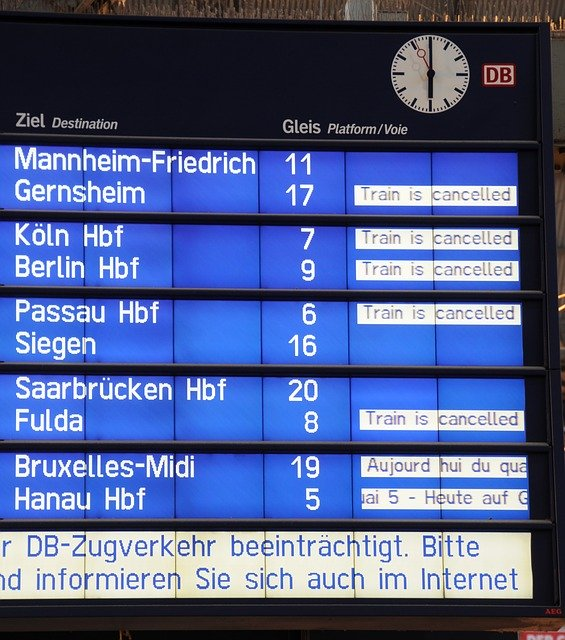
\includegraphics[height=\paperheight]{db.jpg}
      \end{column}
    \end{columns}
  \end{beamercolorbox}
\end{frame}

%%

\begin{frame}{Something different: distributed lotteries}
  Participants \textbf{A, B, \dots, Z} want to agree on a random
  winning ticket.

  \begin{block}{Flawed protocol}
    \begin{itemize}
    \item Each participant \emph{$x$} broadcasts a random string
      \emph{$s_x$};
    \item Winning ticket is \emph{$H(s_A, \dots, s_Z)$}.
    \end{itemize}

    \pause
    
    Cheating participant \textbf{Z} waits to see all other strings,
    then brute-forces \emph{$s_Z$} to win lottery.
  \end{block}
  
  \pause

  \begin{block}{Fixes}
    \begin{itemize}
    \item Make the hash function \textbf{sloooooooooooooooooooooooooooow};
      \begin{itemize}
      \item e.g., participants have 10 minutes to submit $s_x$,
      \item outcome will be known after 20 minutes.
      \end{itemize}
    \item<4-> Make it possible to verify \emph{$w = H(s_A, \dots, s_Z)$} \textbf{fast}.
    \end{itemize}
  \end{block}
\end{frame}

%%

\begin{frame}{Verifiable Delay Functions (Boneh, Bonneau, Bünz, Fisch 2018)}
  \begin{block}{Wanted}
    Function (family) \emph{$f:X\to Y$} s.t.:

    \begin{itemize}
    \item Evaluating $f(x)$ takes \emph{long time}:
      \begin{itemize}
      \item \emph{uniformly} long time,
      \item on almost all random inputs $x$,
      \item even after having seen many values of $f(x')$,
      \item even given \emph{massive number of processors};
      \end{itemize}
    \item Verifying $y=f(x)$ is \emph{efficient}:
      \begin{itemize}
      \item ideally, exponential separation between evaluation and
        verification.
      \end{itemize}
    \end{itemize}
  \end{block}
\end{frame}

%%

\begin{frame}[label=current]{VDFs from RSA groups}
  \begin{columns}
    \begin{column}{0.6\textwidth}
      \begin{block}{Setup}
        \emph{$\Z/N\Z$} with $N=pq$ an RSA modulus, $p,q$ \emph{unknown}\\
        (e.g., generated by some \emph{trusted authority}),
      \end{block}

      \begin{block}{Evaluation}
        With \emph{delay parameter} $\Delta$:
        \begin{align*}
          f:(\Z/N\Z)^\times &\longrightarrow (\Z/N\Z)^\times\\
          x &\longmapsto x^{2^\Delta}
        \end{align*}
        (Conjecturally) takes $\Delta$ squarings.
      \end{block}
    \end{column}
    \begin{column}{0.37\textwidth}
      \centering
      \begin{tikzpicture}[x=2cm,y=2cm]
        \def\crater{29}
        \draw[fill] (360/\crater:1) circle (1pt) +(360/\crater:1em) node {$x$};
        \uncover<2->{
          \draw[fill] (360/\crater : 1) -- (360/\crater*2 : 1)
          circle (1pt) +(360/\crater*2:1em) node {$x^2$};
        }
        \uncover<3->{
          \draw[fill] (360/\crater*2 : 1) -- (360/\crater*3 : 1)
          circle (1pt) +(360/\crater*3:1em) node {$x^4$};
        }
        \uncover<4->{
          \draw[dotted] (360/\crater*3 : 1) arc (360/\crater*3:360/\crater*23:1);
          \draw[fill] (360/\crater*23 : 1) circle (1pt) +(360/\crater*23:1em) node {$x^{2^\Delta}$};
        }
        \uncover<5->{
          \draw[red] (360/\crater : 1) -- node[auto] {$2^\Delta\bmod \varphi(N)$} (360/\crater*23 : 1);
        }
      \end{tikzpicture}

      \medskip
      \uncover<5->{
        If we knew $p,q$, then we could easily verify\dots
      }
      \uncover<6->{
        but we don't!
      }
    \end{column}
  \end{columns}
\end{frame}

%%

\begin{frame}[label=current]{Pietrzak's interactive verification protocol (2018)}
  \emph{Idea:} divide and conquer strategy to prove that
  \[y = x^{2^\Delta}\] 

  (Assume $\Delta$ is a power of $2$)
  \begin{enumerate}
  \item Publish \emph{$z = x^{2^{\Delta/2}}$};
  \item<2-> Receive a random challenge $0 < c < N$,
  \item Recursively prove that:
    \begin{itemize}
    \item \alt<3->{\sout{$z = x^{2^{\Delta/2}}$}}{$z = x^{2^{\Delta/2}}$},
    \item \alt<3->{\sout{$y = z^{2^{\Delta/2}}$}}{$y = z^{2^{\Delta/2}}$},
    \item<3-> \emph{$z^cy = (x^cz)^{2^{\Delta/2}}$}.
    \end{itemize}
  \end{enumerate}

  \medskip
  \begin{description}
  \item[Proof size:] $O(\log(\Delta)\log(N))$.
  \item[Soundness:] Hard to find $w\in(\Z/N\Z)^\times$ of \emph{known
      order} (except $\pm1$).
  \end{description}
\end{frame}

%%

\begin{frame}{Wesolowski's interactive verification protocol (2018)}
  \[y=x^{2^\Delta}\]

  As seen by the verifier:
  \begin{enumerate}
  \item Send a random challenge prime $\ell < B$,
  \item Let \emph{$2^\Delta = q\ell + r$},
  \item Receive \emph{$z = x^q$},
  \item Check that \emph{$z^\ell x^r = y$}.
  \end{enumerate}

  \bigskip
  \begin{description}
  \item[Proof size:] $O(\log(N))$.
  \item[Soundness:] \textit{ad hoc} security assumption.
  \end{description}
\end{frame}

%%

\begin{frame}[label=current]{Additional remarks}
  \begin{block}{On interactivity}
    Proofs can be made \emph{non-interactive} using the standard
    Fiat-Shamir transform.
  \end{block}

  \begin{block}{Removing trusted third parties}
    \begin{itemize}
    \item RSA setup requires \emph{trusted generation of $N=pq$}
      (single or distributed authority);
    \item The only property used by the VDFs is that \emph{the order
        of $(\Z/N\Z)^\times$ is unknown};
    \item Can adapt the protocol to any cryptographic \emph{group of
        unknown order}:
      \begin{itemize}
      \item e.g., \emph{quadratic imaginary class groups} of unknown
        order can be publicly generated with no trusted setup!
      \end{itemize}
    \end{itemize}
  \end{block}
\end{frame}

%%

\begin{frame}[label=current]{Quadratic imaginary WHAT?! {\small(Where things start going south\dots)}}
  \large
  
  Quadratic imaginary class groups are:
  \begin{itemize}
  \item<+-> Extremely cool objects in number theory,
  \item<+-> Commutative Galois groups of some field extensions of
    \emph{$\Q(\sqrt{-D})$},
  \item<+-> Somehow related to the ideals of \emph{$\Z[\sqrt{-D}]$},
  \item<+-> Related to elliptic curves and isogenies by the theory of
    \emph{complex multiplication}.
  \end{itemize}
\end{frame}

%%

\begin{frame}{Where have I seen this before?}
  \begin{columns}
    \begin{column}{0.6\textwidth}
      \begin{uncoverenv}<2->
        \begin{block}{Isogeny cycles}
          \begin{itemize}
          \item Vertices are \emph{elliptic curves}:
            \begin{itemize}
            \item Ordinary,
              \hfill\uncover<4->{\emph{Couveignes--Rostovtsev--Stolbunov}}
            \item Supersingular $/\F_p$.
              \hfill\uncover<4->{\emph{CSIDH}}
            \end{itemize}
          \item Edges are \emph{horizontal isogenies}.
          \item<3-> All curves have the same \emph{endomorphism ring}
            isomorphic to some $\Z[\sqrt{-D}]$.
          \item<3-> The \emph{class group} of $\Z[\sqrt{-D}]$ acts upon the
            cycle:

            \smallskip
            \begin{tabular}{r c l}
              isogeny & ~$\leftrightarrow$~ & ideal\\
              endomorphism  & ~$\leftrightarrow$~ & principal ideal\\
              degree & ~$\leftrightarrow$~ & norm\\
              dual & ~$\leftrightarrow$~ & complex conjugate\\
              cycle size & ~$\leftrightarrow$~ & order of the ideal
            \end{tabular}
          \end{itemize}
        \end{block}
      \end{uncoverenv}
    \end{column}
    \begin{column}{0.4\textwidth}
      \centering
      \begin{tikzpicture}[x=2cm,y=2cm]
        \def\crater{17}
        \foreach \i in {0,...,16} {
          \draw[fill] (360/\crater*\i:1) circle (1pt)
          +(360/\crater*\i:1em) node {\alt<2->{$E_{\i}$}{$x^{2^{\i}}$}};
          \draw (360/\crater*\i : 1) edge[bend right] (360/\crater*\i+360/\crater : 1);
        }
      \end{tikzpicture}
    \end{column}      
  \end{columns}
\end{frame}

%%

\begin{frame}{Slooooooooooooooooooooooooooooooooow isogenies (Asiacrypt '19)}
  \begin{columns}
    \begin{column}{0.6\textwidth}
      \begin{block}{Setup}
        With \emph{delay parameter} $T$:
        \begin{itemize}
        \item A laaaaaaaaaaaaaaaaaaaaaaaarge isogeny cycle,
        \item<2-> A \emph{starting curve} $E_0$,
        \item<2-> An isogeny \emph{$\phi:E_0\to E_T$} of degree \emph{$2^T$}.
        \end{itemize}
      \end{block}

      \begin{uncoverenv}<3->
        \begin{block}{Evaluation}
          $\phi$ \textbf{is} the VDF:
          \begin{align*}
            \phi:E_0(\F_p) &\longrightarrow E_T(\F_p)\\
            P &\longmapsto \phi(P)
          \end{align*}
          Conjecturally, no faster way than \emph{composing degree $2$
            isogenies}.
        \end{block}
      \end{uncoverenv}
    \end{column}
    \begin{column}{0.37\textwidth}
      \centering
      \begin{tikzpicture}[x=2cm,y=2cm]
        \def\crater{29}
        \draw[fill] (360/\crater:1) circle (1pt) +(360/\crater:1em) node {$E_0$};
        \draw[fill] (360/\crater : 1) -- (360/\crater*2 : 1)
        circle (1pt) +(360/\crater*2:1em) node {$E_1$};
        \draw[fill] (360/\crater*2 : 1) -- (360/\crater*3 : 1)
        circle (1pt) +(360/\crater*3:1em) node {$E_2$};
        \draw[dotted] (360/\crater*3 : 1) arc (360/\crater*3:360/\crater*23:1);
        \draw[fill] (360/\crater*23 : 1) circle (1pt) +(360/\crater*23:1em) node {$E_T$};
        \uncover<4->{
          \draw (0,0) node[anchor=center] {\Large\alert{\alt<5->{Pairings!}{How to verify?}}};
        }
      \end{tikzpicture}
    \end{column}
  \end{columns}
\end{frame}

%%

\begin{frame}{For concreteness}
  \emph{Elementary step:}
  \medskip
  
  \hspace{2em} RSA: \hfill $x \longmapsto x^2\mod N$ \hspace{4em}

  \vfill
  \hspace{2em} Isogenies: \hfill $\displaystyle x \longmapsto \frac{(x+1)^2}{4\alpha_ix}\mod p$ \hspace{4em}\strut\\
  {\hspace{2em}\normalsize\color{gray} ($\alpha_1,\dots,\alpha_T$ correspond to the isogeny steps)}

  \vfill
  \begin{description}
  \item[Typical parameters:] \emph{$\log_2 p \approx 1500$} gives
    security similar to $\log_2 N \approx 2048$.
  \item[Huge storage:] we estimate \emph{$\approx$ 16TiB} for storing
    $(\alpha_1,\dots,\alpha_T)$ for a 1 hour delay!
  \end{description}
\end{frame}

%%

\begin{frame}{Comparison}
  \begin{tabular}{l | c c | c c | c c}
    & \multicolumn{2}{c|}{Wesolowski} & \multicolumn{2}{c|}{Pietrzak} & \multicolumn{2}{c}{Ours}\\
    & RSA & class group & RSA & class group & $\F_p$ & $\F_{p^2}$\\
    \hline
    proof size    & $O(1)$ & $O(1)$ & $O(\log(T))$ & $O(\log(T))$ & --- & ---\\
    aggregatable  & yes & yes & yes & yes & --- & ---\\
    watermarkable & yes & yes & yes & yes & (yes) & (yes)\\
    perfect soundness & no & no & no & no & yes & yes\\
    \textit{long} setup & no & no & no & no & \alert{yes} & \alert{yes}\\
    trusted setup & \alert{yes} & no & \alert{yes} & no & \alert{yes} & \alert{yes}\\
    best attack   & $L_N(1/3)$ & $L_N(1/2)$ & $L_N(1/3)$ & $L_N(1/2)$ & $L_p(1/3)$ & $L_p(1/3)$\\
    quantum annoying & no & (yes) & no & (yes) & no & yes\\
  \end{tabular}
\end{frame}

%%

\begin{frame}{Applications}
  \begin{block}{Randomness beacons}
    \begin{description}
    \item[Goal:] Generate a public stream of provably random numbers.
    \item[Standard technique:] Hash output of public high entropy
      sources (e.g.: stock market, weather, \dots) at regular
      intervals (epochs).
    \item[Risk:] Close to the end of the epoch, adversary manipulates
      the data (e.g., buys stock) repeatedly until they get the
      desired alea.
    \item[Fix:] Run the hashed value through a VDF with delay longer
      than the epoch.
    \end{description}
  \end{block}

  \begin{block}{Proofs of Stake/Space}
    \begin{description}
    \item[Goal:] Elect epoch leader(s) in PoS blockchains.
    \item[Standard technique:] PoS are assigned a ``quality'' (e.g.:
      hash of the PoS), the higher quality gets elected as leader.
    \item[Disadvantage:] Requires synchronization of miners.
    \item[Fix (Chia):] Run the PoS through a VDF with delay
      proportional to quality.
    \end{description}
  \end{block}
\end{frame}

%%

\begin{frame}{VDF Craze}
  Blockchains  are investing big in VDFs

  \begin{description}
  \item[VDF Alliance\footnote{\url{https://www.vdfalliance.org/}}:]
    formed by Etherereum, Protocol Labs, Tezos, Interchain,
    Supranational.
  \item[VDF competitions] (cash prizes in the order of 100k\$):
    \begin{itemize}
    \item RSA-based, run by VDF
      Alliance\footnote{\url{https://supranational.atlassian.net/wiki/spaces/VA/pages/36569208/FPGA+Competition}}.
      \begin{itemize}
      \item Squaring modulo $N$,
      \item Distributed generation of RSA numbers.
      \end{itemize}
    \item Class group based, run by
      Chia\footnote{\url{https://github.com/Chia-Network/vdf-competition/}}.
      \begin{itemize}
      \item Class number computation.
      \item Squaring in class groups.
      \end{itemize}
    \end{itemize}
  \item[More resources:] \url{https://vdfresearch.org/}.
  \end{description}
\end{frame}

%%

\begin{frame}[plain]
  \begin{beamercolorbox}[sep=0.1px,center,wd=\paperwidth,ht=\paperheight]{palette tertiary}
    \begin{columns}
      \begin{column}{0.55\textwidth}
        \Huge\centering More Delay\\ Functions
      \end{column}
      \begin{column}{0.45\textwidth}
        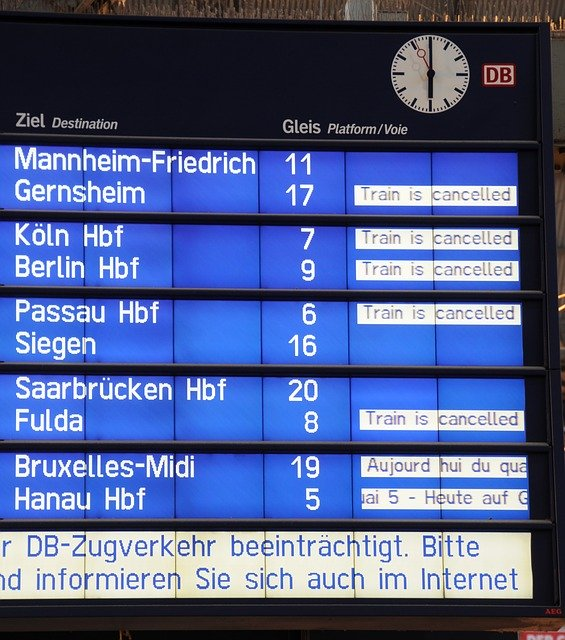
\includegraphics[height=\paperheight]{db.jpg}
      \end{column}
    \end{columns}
  \end{beamercolorbox}
\end{frame}

%%

\begin{frame}{Watermarking}
  \def\Emid{E_{\mathrm{mid}}}
  \def\emid{e_{\mathrm{mid}}}
  \begin{description}
  \item[Goal:] reward evaluator of the VDF for their effort.
  \item[Watermarking:] issue proof of evaluation \emph{tied to
      evaluator identity}
  \item[In group-based,] easy: hash identity in the Pietrzak/Wesolowski
    non-interactive proof.
  \item[In isogeny-based:] there is no proof, a workaround is needed:
  \end{description}

  \centering
  \begin{tikzpicture}[x=5cm]
    \node (E) at (0,0) {$E$};
    \node (Em) at (1,0) {$\Emid$};
    \node (E1) at (2,0) {$E'$};
    
    \draw[auto,->] (E1) edge[bend right] node {$\hat\phi_1$} (Em)
    (Em) edge[bend right] node {$\hat\phi_2$} (E)
    (E1) edge[bend left] node[swap] {$\hat\phi = \hat\phi_2\circ\hat\phi_1$} (E);
  \end{tikzpicture}

  \begin{description}
  \item[Secret key:] scalar $s\in\Z/N\Z$,
  \item[Public key:] $s\phi(P) \in E'$ \textcolor{gray}{(+ proof of exponent knowledge)},
  \item[Proof of work:] $s\hat\phi_1(Q) \in \Emid$,
  \item[Properties:] blind (can be checked before the computation is
    complete).
  \end{description}
\end{frame}

%%

\begin{frame}{Homomorphic time-lock puzzles}
  \begin{block}{Voting, reloaded}
    \begin{itemize}
    \item Each bidder encrypts bid with a TL puzzle;
    \item At the end of the auction each well behaved bidder reveals
      its trapdoor;
    \item Other bids are opened with SlowKDF.
    \end{itemize}

    \begin{description}
    \item[Problem:] What if 100k participants do not reveal the
      trapdoor?
    \item[Solution:] Combine homomorphically the votes, run SlowKDF
      only once.
    \end{description}
  \end{block}

  \begin{block}{Malavolta, Thyagarajan 2019}
    \begin{itemize}
    \item Generalization of the \emph{RSA-based TL puzzle}, insipired
      by \emph{Paillier}.
      \begin{itemize}
      \item Additively homomorphic version (good for voting),
      \item Multiplicatively homomorphic version.
      \end{itemize}
    \item Generic fully homomorphic construction based on \emph{FHE + iO}.
      \begin{itemize}
      \item In particular, totally impractical for auctions.
      \end{itemize}
    \end{itemize}
  \end{block}
\end{frame}

%%

\begin{frame}{Delay encryption {\small(soon to be rejected at Crypto)}}
  \begin{description}
  \item[Goal:] Same problem as in homomorphic TL puzzles.
  \item[Solution:] A TL puzzle \emph{without trapdoor}.
    \begin{itemize}
    \item Requires a \emph{randomness beacon} to avoid precomputation
      attacks.
    \end{itemize}
  \item[Idea:] Chimera of \emph{Isogeny VDF} and \emph{Boneh-Franklin
      IBE} {\color{gray}\small(only known construction)}.
  \end{description}

  \bigskip
  \centering
  \begin{tabular}{c c c}
    \textbf{Bidder} && \textbf{Notaries}\\
                    && Publish auction key \emph{$Q = \mathcal{H}(\mathsf{sid})$}\\
                    && start evaluating \emph{$\hat\phi(Q)$}\\
    samples random \emph{$s\in\Z/N\Z$}\\
    computes \emph{$k = e(\phi(P), Q)^s$}\\
    encrypts offer \emph{$o_k = \mathrm{Enc}_{k}(o)$}\\
    \hfill sends \emph{$(o_k,sP)$} & $\longrightarrow$\\
                    && $\vdots$\\
                    && compute \emph{$k = e(sP, \hat\phi(Q))$}\\
                    && decrypt \emph{$o_k$}
  \end{tabular}
\end{frame}

%%

\begin{frame}{(My favorite) open questions}
  \begin{itemize}
  \item<+-> Understand the impact of large memory requirements in
    evaluation; is a time/memory trade-off reasonable?
  \item<+-> Remove trusted setup:
    \begin{itemize}
    \item Hash into the supersingular set, or
    \item Construct ordinary pairing friendly curves with large
      discriminant.
    \end{itemize}
  \item<+-> Explore more advanced pairing+delay constructions.
  \item<+-> Spend millions on dedicated hardware for $2$-isogenies.
  \end{itemize}

  \bigskip
  \begin{uncoverenv}<+->
    \begin{center}
      \Large Just Add Isogenies\texttrademark!
    \end{center}
  \end{uncoverenv}
\end{frame}

%%

\begin{frame}[plain]
  \centering
  \begin{tikzpicture}[remember picture,overlay]
    \begin{scope}[xscale=1.7,yshift=-15,opacity=0.8]
      \def\crater{12}
      \def\jumpa{-8}
      \def\jumpb{9}
      \def\diam{5cm}

      \foreach \i in {1,...,\crater} {
        \draw[blue] (360/\crater*\i : \diam) to[bend right] (360/\crater*\i+360/\crater : \diam);
        \draw[red] (360/\crater*\i : \diam) to[bend right] (360/\crater*\i+\jumpa*360/\crater : \diam);
        \draw[green] (360/\crater*\i : \diam) to[bend right=50] (360/\crater*\i+\jumpb*360/\crater : \diam);
      }
    \end{scope}
    
    \draw (0,0) node{\Huge\bf Thank you};
    \draw (0,-1.6) node{\large
\includegraphics[height=0.9em]{twitter.png}~\href{https://twitter.com/luca_defeo}{@luca\_defeo}};
  \end{tikzpicture}
\end{frame}

\end{document}


% LocalWords:  Isogeny abelian isogenies hyperelliptic supersingular Frobenius
% LocalWords:  isogenous
